\documentclass[a4paper,12pt,fleqn]{scrartcl}%fleqn pour aligner les equations à gauche
\usepackage{../../Styles/Eval}


\newcommand{\chnum}{Chapitre 11}
\newcommand{\chtitle}{Mouvement}
\newcommand{\dtype}{DS 3}

\begin{document}
\maketitle
\section{Décollage d'un hélicopter}
Un hélicopter effectue une opération de secours. Avant de décoller, ses pales tournent à vitesse constante. Après le décollage, l'hélicoptère s'élève verticalement au-dessus du sol à vitesse constante.
\begin{question}
    \begin{enumerate}
    \item Définir les systèmes, supposés ponctuels, qui décrivent dans le référentiel terrestre :
    \begin{enumerate}
        \item un mouvement circulaire uniforme avant le décollage
        \item un mouvement rectiligne uniforme après le décollage
    \end{enumerate}
    \item Décrire le mouvement de chaque système après le décollage, dans le référentiel de la cabine de l'hélicoptère.
    \item Expliquer pourquoi, après décollage, il n'est pas judicieux de modéliser l'hélicoptère par un point pour étudier son mouvement.
\end{enumerate}
\end{question}
\noindent\begin{minipage}{.6\linewidth}
    Le Sud-Aviation SA315B Lama est un hélicoptère de transport français, détenteur du record d'altitude en hélicoptère à \SI{12422}{m}. Son rotor (comprenant les pales) ont un diamètre de \SI{11,02}{m} et une vitesse de rotation d'environ \SI{1600}{tour/min}.
\begin{question}
    \begin{enumerate}
        \setcounter{enumi}{3}
    \item Exprimer la distance parcourue par l'extrémité d'une pale pendant un tour.
    \item Calculer la la vitesse de déplacement de l'extrémité d'une pale en \unit{\meter\per\second}.
\end{enumerate}
\end{question}
\end{minipage}\hspace{1em}\begin{minipage}{.38\linewidth}
    \centering
    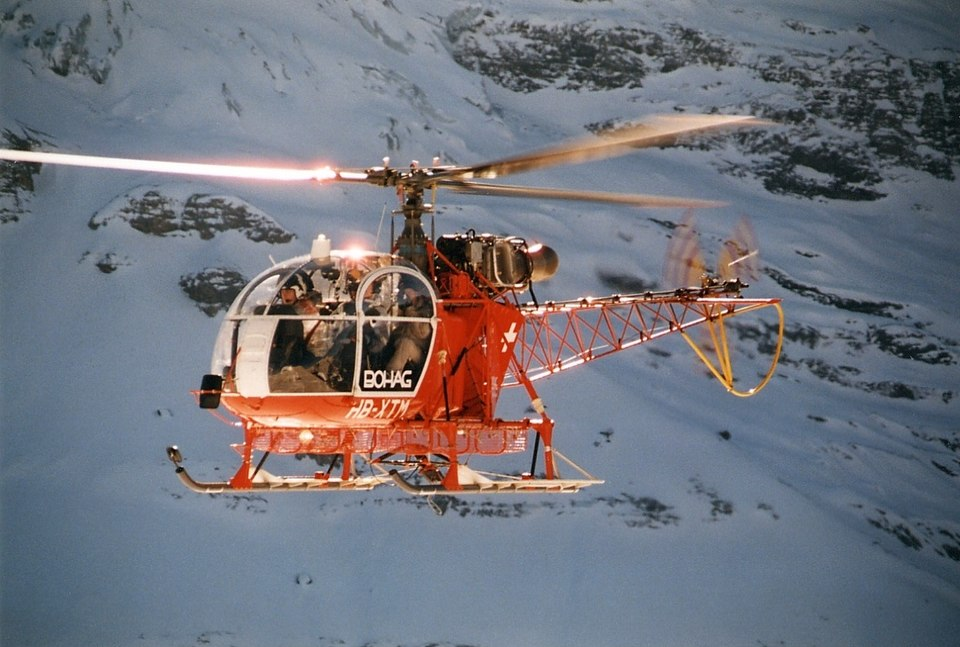
\includegraphics[width=\linewidth]{Resssources/Lama_helico.jpg}
\end{minipage}
\vspace{5em}
\begin{center}
    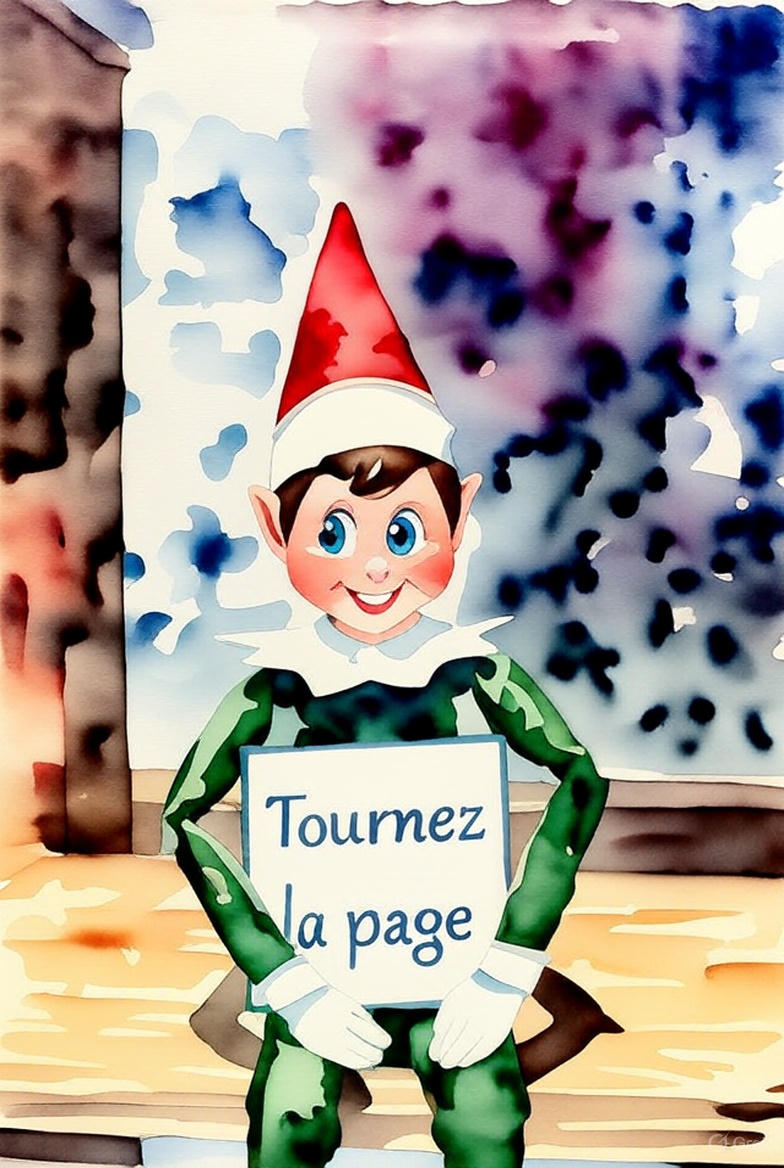
\includegraphics[width=.2\linewidth]{Resssources/elf_tourner.jpg}
\end{center}

\newpage
\section{Seul sur Mars}
Dans ke film \textit{Seul sur Mars}, Mark Watney s'évanouit dans la fusée chargée de le ramener au vaisseau principal. Son collègue commente : "Il vient de se prendre \SI{13}{g}, laissez-lui deux minutes". Avant de partir en expédition, les astronautes sont préparés à subir de fortes accélérations, communément quantifiées en \unit{\gram}. Sur Terre, lorsqu'une fusée "monte à \SI{1}{g}", cela signifie que sa vitesse augmente de \SI{10}{\meter\per\second}, en une seconde.

\begin{question}
    \begin{minipage}{.48\linewidth}
        \begin{enumerate}
            \item Calculer les valeurs des vitesse $v_0$ et $v_4$.
            \item Représenter les vecteurs vitesse $\vv{v_0}$ et $\vv{v_4}$. Echelle : $\SI{1}{cm}\leftrightarrow\SI{50}{cm}$
            \item Démontrer que la variation de la vitesse entre les instants $t_0$ et $t_4$ vaut : $$\Delta v = v_4 -v_0 = \SI{260}{\meter\per\second} $$
            \item Quel est l'intervalle de temps $\Delta t$ séparant la position $t_0$ et $t_4$ ?
            \item L'accélération $a$ peut se calculer avec la formule : $$a = \dfrac{v_4-v_0}{\Delta t}$$ Calculer l'accélérationde Mark.
            \item Comparer cette accélération avec la valeur de $g$. La phrase "Il vient de se prendre \SI{13}{g}", vous parait-elle correcte ?
        \end{enumerate}
    \end{minipage}
    \begin{minipage}{.5\linewidth}
    \centering
    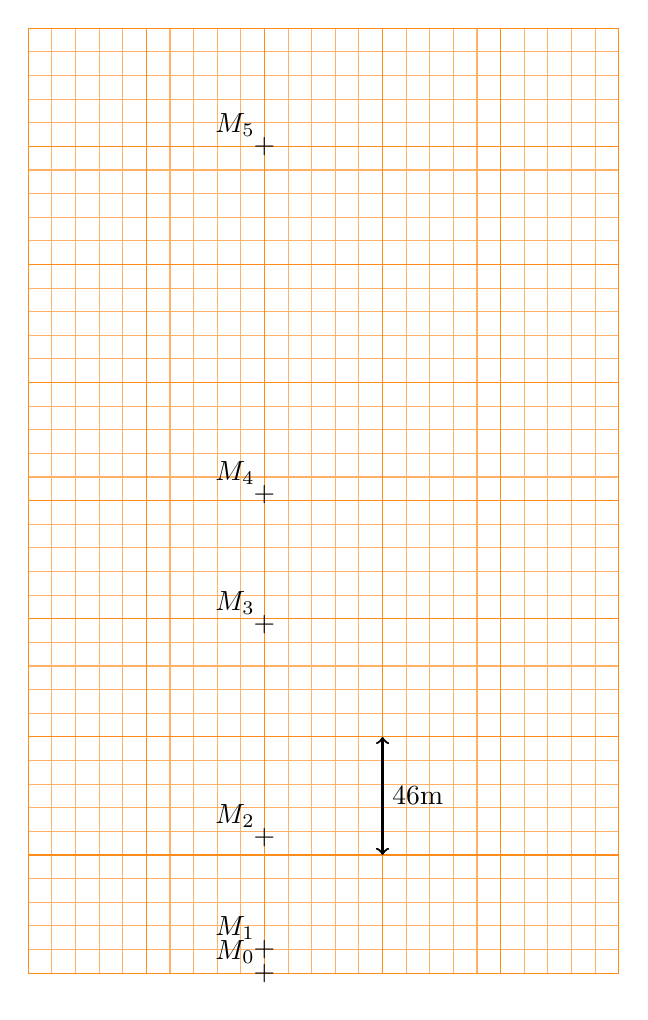
\begin{tikzpicture}[scale=1.5]
    \draw[orange!60] (0,0) grid[step=.2] (5,8);
    \draw[orange!90] (0,0) grid (5,8);
    \draw[<->,thick](3,1) to (3,2);
    \node[right] at(3,1.5){\SI{46}{m}};
    
    \foreach \k [count=\xi] in {0,.2,1.15,2.95,4.05,7}{
        \pgfmathsetmacro\m{\xi-1}
        \draw (2,\k) node{+};
        \node[above left] at(2,\k){$M_{\pgfmathprintnumber{\m}}$};
        
    }
    \end{tikzpicture}

    On a représenté les positions successivement occupées par Mark. La durée séparant chaque position est égale à \SI{0,50}{\second}.
    \end{minipage}
\end{question}

    

\end{document}